\section{Residue Class Potential Model}
Fix a modulus \( m \in \mathbb{Z}_{>0} \), and let \( \mathbb{Z}_{m} = \{0, 1, \dots, m-1\} \). Define a potential \( V: \mathbb{Z}_{m} \to \mathbb{R}_{\geq 0} \) reflecting prime density modulo \( m \). For \( m = 12 \), residue classes \( \{1, 5, 7, 11\} \) are prime-rich (e.g., no primes \(\equiv 0 \modm\)).

We define:
\[
V(x) =
\begin{cases}
V_{\text{low}} = 0.5, & \text{if } x \in \{1, 5, 7, 11\}, \\
V_{\text{high}} = 1.5, & \text{otherwise}.
\end{cases}
\]

\begin{figure}[t]
\centering
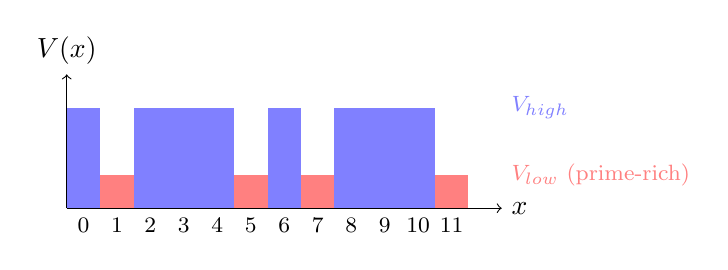
\begin{tikzpicture}[scale=0.85]
    % Draw the initial potential function
    \draw[->] (0,0) -- (6.5,0) node[right] {$x \modm$};
    \draw[->] (0,0) -- (0,2) node[above] {$V(x)$};
    
    % Draw the potential values
    \foreach \x/\label in {0/0, 1/1, 2/2, 3/3, 4/4, 5/5, 6/6, 7/7, 8/8, 9/9, 10/10, 11/11} {
        \node[below] at (0.5*\x + 0.25, 0) {\footnotesize \label};
    }
    
    % Draw the potential bars
    \foreach \x in {0, 2, 3, 4, 6, 8, 9, 10} {
        \fill[blue!50] (0.5*\x, 0) rectangle (0.5*\x + 0.5, 1.5);
    }
    \foreach \x in {1, 5, 7, 11} {
        \fill[red!50] (0.5*\x, 0) rectangle (0.5*\x + 0.5, 0.5);
    }
    
    % Add legend
    \node[red!50, right] at (6.5,0.5) {\footnotesize $V_{low}$ (prime-rich)};
    \node[blue!50, right] at (6.5,1.5) {\footnotesize $V_{high}$};
\end{tikzpicture}
\caption{Initial potential $V(x)$ defined on residue classes modulo $m=12$, with lower values for prime-rich classes.}
\label{fig:initial_potential}
\end{figure}

% NEW ILLUSTRATION FOR PRIME DISTRIBUTION
\begin{figure}[t]
\centering
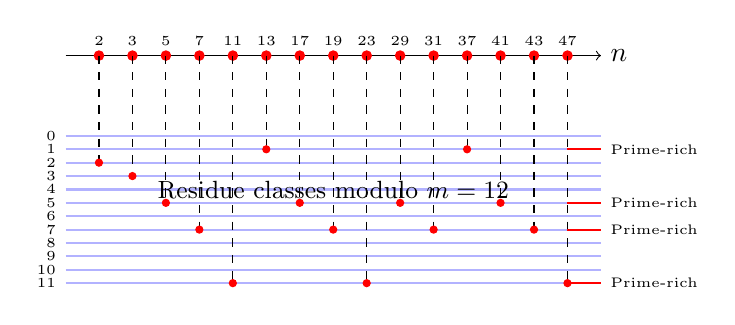
\begin{tikzpicture}[scale=0.85]
    % Draw the number line with primes
    \draw[->] (0,2) -- (8,2) node[right] {$n$};
    \foreach \x/\p in {1/2, 2/3, 3/5, 4/7, 5/11, 6/13, 7/17, 8/19, 9/23, 10/29, 11/31, 12/37, 13/41, 14/43, 15/47} {
        \filldraw[red] (\x*0.5, 2) circle (2pt);
        \node[above] at (\x*0.5, 2) {\tiny \p};
    }
    
    % Draw the residue classes
    \foreach \i in {0,...,11} {
        \draw[thick, blue!30] (0,0.8-0.2*\i) -- (8,0.8-0.2*\i);
        \node[left] at (0,0.8-0.2*\i) {\tiny $\i \modm$};
    }
    
    % Connect primes to their residue classes
    \foreach \x/\p/\r in {1/2/2, 2/3/3, 3/5/5, 4/7/7, 5/11/11, 6/13/1, 7/17/5, 8/19/7, 9/23/11, 10/29/5, 11/31/7, 12/37/1, 13/41/5, 14/43/7, 15/47/11} {
        \draw[dashed] (\x*0.5,2) -- (\x*0.5,0.8-0.2*\r);
        \filldraw[red] (\x*0.5,0.8-0.2*\r) circle (1.5pt);
    }
    
    % Highlight the prime-rich residue classes
    \foreach \r in {1,5,7,11} {
        \node[right] at (8,0.8-0.2*\r) {\tiny Prime-rich};
        \draw[red, thick] (7.5,0.8-0.2*\r) -- (8,0.8-0.2*\r);
    }
    
    % Add caption under the figure
    \node at (4,0) {\small Residue classes modulo $m=12$};
\end{tikzpicture}
\caption{Distribution of prime numbers in residue classes modulo $m=12$, showing how primes $>3$ are distributed only in classes $\{1,5,7,11\}$, making these "prime-rich" classes.}
\label{fig:prime_distribution_detailed}
\end{figure}

\subsection*{Connection to Zeta Function}
The potential \( V(x) \) approximates prime density in residue classes, which influences the zeta function's zeros via Dirichlet \( L \)-functions. The explicit formula for \(\zs\) relates the zeros' imaginary parts to prime powers:
\[
\sum_{\rho} e^{i t \Im(\rho)} \sim \sum_p \sum_{k=1}^\infty \frac{\log p}{p^{k/2}} e^{i t k \log p},
\]
where \( \rho \) are non-trivial zeros. By encoding prime density in \( V(x) \), we shape the operator's spectrum to approximate \( \Im(\rho) \).